% Rules for the HuroCup Sprint Competition
% Jacky Baltes <jacky@cs.umanitoba.ca> 

\documentclass[12pt]{hurocup}

\newcommand{\thisyear}{2010}

\newcommand{\HuroCup}{\textsc{HuroCup}}


\begin{document}

\title{\HuroCup: Robot Sprint\ \\
  Laws of the Game \thisyear}

\author{Jacky Baltes\\
Autonomous Agents Laboratory\\
University of Manitoba\\
Winnipeg, Manitoba\\
Canada, R3T 2N2\\
Email: jacky@cs.umanitoba.ca\\
WWW: http://www.cs.umanitoba.ca/\~{ }jacky\\[5mm]
Kuo-Yang Tu\\
National Kaohsiung First University of Science and Technology\\
Kaohsiung City, R. O. C.\\
Email: tuky@ccms.nkfust.edu.tw\\
}

\maketitle

\begin{center}
 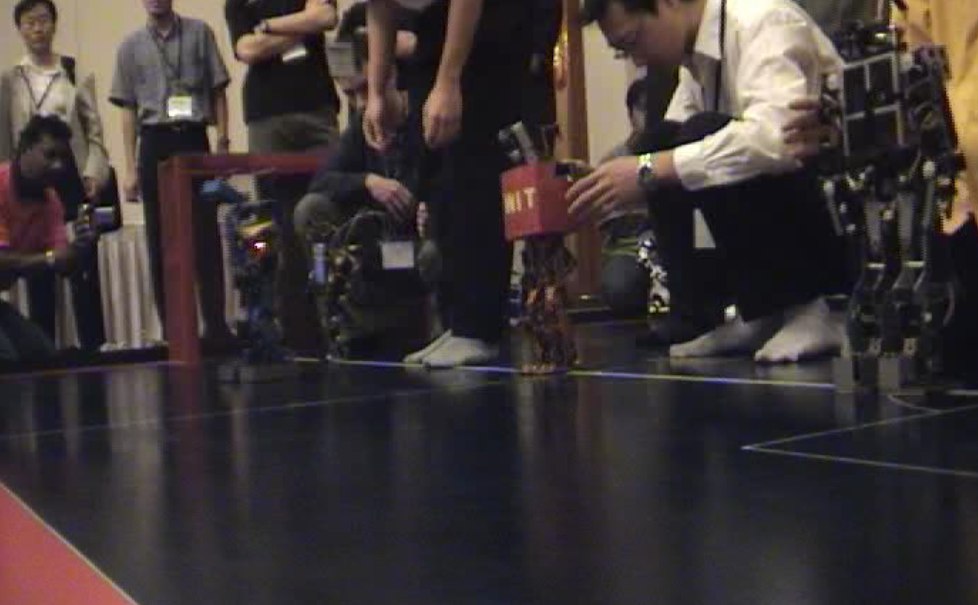
\includegraphics[width=0.7\linewidth]{Figures/sprint-life}
\end{center}

\begin{abstract}
The following rules and regulations govern the game of the Robot Sprint
event in \HuroCup, a robotic game and robotics benchmark problem for
humanoid robots.
%
\end{abstract}

\section*{Latest Version of the Rules for \HuroCup}
\label{sec:updates}

The latest official version of the rules of the game for \HuroCup\ is
always available from the FIRA \HuroCup\ website (http://www.fira.net).

\newpage

\section{Robot Sprint}
\label{sec:robot-sprint}

The robot sprint challenge is a sprint event for humanoid robots. The
goal is for the robots to move as quickly as possible from a start
line to the end line for a series of segments.

\section{Laws of the Game: Sprint}
\label{sec:laws-sprint}

The following laws describe the specifics of the robot sprint event. For
general specifications relevant to all \HuroCup\ events (e.g., robot
dimensions, playing field and lighting, responsibility of the
referees) please refer to the general \HuroCup\ laws.

\law[RD]{The Field of Play}
\label{law:field-of-play}

\begin{lawlist}[RD]

\item The dimensions of the playing field are at least 430 by
  200cm. 
  
\item The playing field consists of a race track that run the whole
  width of the playing field.

\item There are two zones on the ends of the race track. The zones are
  marked by lines parallel to the goal lines. Please refer to
  Fig.~\ref{fig:sprint}.

\item The width of the zones is the width of the playing field and the
  length of the zones is at least 30cm.
  \begin{figure}
    \begin{center}
      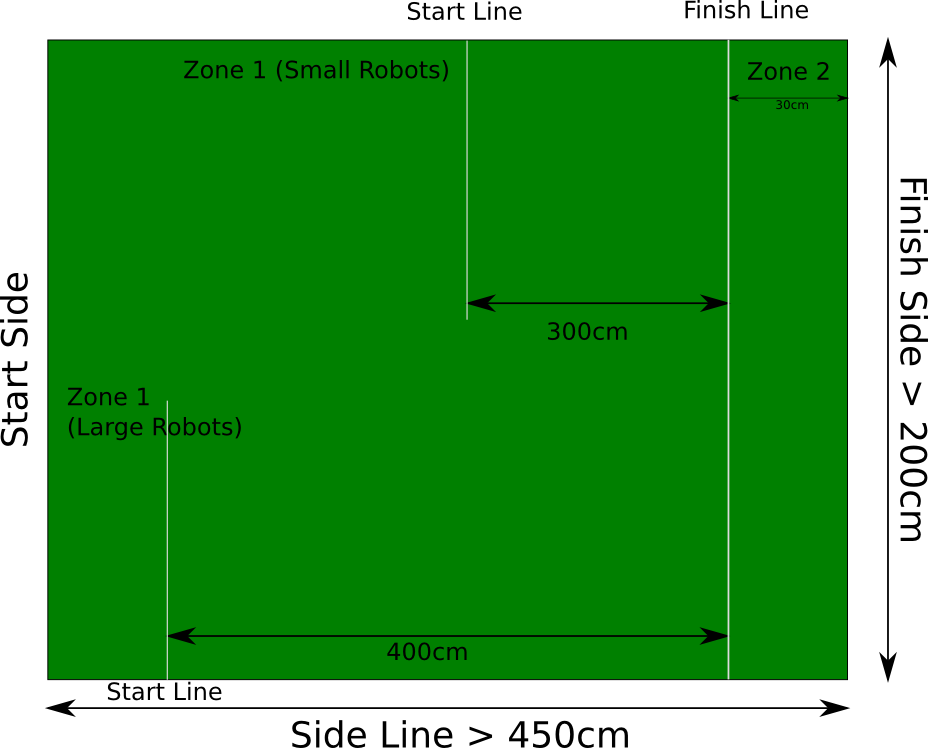
\includegraphics[width=0.7\textwidth]{Figures/sprint}
    \end{center}
    \caption{The field of play for robot sprint}
    \label{fig:sprint}
  \end{figure}
  
\item There length of the race tracks depends on the height of the
  robots. The race tracks are parallel to the side lines.
  \begin{enumerate}
  \item The length of the race track for small robots
    is 300cm.
  \item The length of the race track for large robots
    is 400cm.
  \end{enumerate}

\item All lines are marked with are white and have a width between 5mm
  and 15mm.
  
\item Teams may place small coloured markers in the end zones to guide
  the robot as long as they do not interfere with other teams.
\end{lawlist}

\law[RD]{Number of Robots}

\begin{lawlist}[RD]
\item A single robot competes in a match.
\end{lawlist}

\law[RD]{The Players}

Please refer to the general \HuroCup\ laws for a description of
the players.

\law[RD]{The Referee}

Please refer to the general \HuroCup\ laws for a description of
the referee.

\law[RD]{The Assistant Referee}

Please refer to the general \HuroCup\ laws for a description of
the assitant referee.

\law[RD]{Game Play}

\begin{lawlist}[RD]
  
\item At the beginning of the competition, all robots must be behind
  the start line (i.e., in Zone 1) of their respective categories.

\item The referee will signal the start of the competition by blowing
  the whistle. After the referee blows the whistle, the robots walk
  forwards towards the end of segment 1 (i.e., zone 2).

\item A robot is not allowed to leave the playing field as defined
  in~\ref{law:field-of-play}.  If a robot leaves the playing field, it
  must be moved back to the start zone.

\item A robot has crossed the end line of one segment when either
  foot of the robot crosses the finish plane and touches the ground in
  the respective zone. The finish plane is the plane which intersects
  the playing field at a 90 degree angle at the back of the finish
  line.
  
\item After the robot has crossed the finish line of the first segment
  (i.e., the robot has reached Zone 2), the robot must walk backwards
  towards the end line for segment 2 (i.e., Zone 1).
  
\item A robot is walking backwards if the difference of the robot's
  current orientation to its orientation when positioned at the start
  line is at most 90 degrees in either direction.
  
\item The robot must move forward towards in segment 1, and backwards
  in segment 2.
  
\item Each robot may have at most one human handler associated with
  it.

\item \label{rd-handler3} The human handlers are not allowed to
  interfere in any way with other robots, the referee, or other human
  handlers.

\item \label{rd-handler4} A human handler may only enter the playing
  field or touch his/her robot with the permission of the referee.

\item The handler shall remove his/her assigned robot as soon as
  possible from the respective end zone after it has crossed the
  finish line.

\item Any robot that either leaves the playing field or breaks down
  may be moved by a human helper and placed again behind the start
  line. This is subject to laws~\ref{rd-handler3}
  and~\ref{rd-handler4}.

\item The end of the competition is signaled by the referee by blowing
  the whistle a second time. The referee terminates the competition
  if
  \begin{itemize}
  \item the maximum duration of the competition (10 minutes) has
    elapsed.
  \item all robots have crossed the finish line of the backward
    segment,
  \item no more active robots remain in the competition.
  \end{itemize}

\end{lawlist}

\law[RD]{Fouls and Misconduct}

\begin{lawlist}[RD]
\item A robot is not allowed to interfere with another robot in any
  way.

\item Light contact: Should the contact between two robots be light
  and infrequent, then the referee uses the following rules:
  \begin{enumerate}

  \item should a contact occur between two robots where one robot is
    deemed responsible by the referee for the offense (for example, the
    other robot is stationary), then the offending robot must be moved
    back behind the start line and continue with segment 1. The robot
    may then continue in the competition.

  \item if both both robots are moving, then the referee will have
    both robots moved behind the start line by the human
    handlers. Once both robots have been moved behind the start line,
    they may then continue in the competition by restarting segment 1.
  \end{enumerate}

\item The referee may use the penalties described in the general laws
of \HuroCup\ accordingly.

\end{lawlist}

\law[RD]{Method of Scoring}
\label{rd:scoring}

\begin{lawlist}[RD]

\item Robots are awarded points based on the last segment that the
robot completed successfully as well as the order in which they
crossed the end line of the last segment.

\item All robots that have not crossed the finish line of at least the
  first segment are automatically awarded no rank and $0$ points.

\item Among the robots that have crossed the finish line of the at
  least the first segment, the robots are ranked (i.e., 1st place, 2nd
  place) based on the maximum segment number that the robot completed
  successfully. All robots with the same maximum segment number are
  ranked based on the faster time to complete that segment.

\item The point allocation for robots is as follows:
  \begin{itemize}
  \item The first ranked robot is awarded $10$ points.
  \item The second ranked robot is awarded $8$ points.
  \item The third ranked robot is awarded $6$ points.
  \item The fourth, fifth, sixth, and seventh place robots are awarded
    $4$,$3$,$2$, and $1$ point respectively.  A summary of the point
    allocation for placings is shown in table~\ref{point-allocation}.

    \begin{table}
      \begin{center}
        \begin{tabular}{l|l}
          \hline
          Place & Points scored \\
          \hline
          1 (Winner) & 10 \\
          2          & 8 \\
          3          & 6 \\
          4          & 4 \\
          5          & 3 \\
          6          & 2 \\
          7          & 1 \\
          8, 9, ...  & 0 \\
          \hline
        \end{tabular}
      \end{center}
      \caption{Point allocation for placings in the \HuroCup\ events.}
      \label{point-allocation}
    \end{table}
  \end{itemize}

\item In case of a tie between $n$ robots with rank $k$, all robots
 will be awarded rank $k$ and receive the average of the scores for
 ranks $k$ to $k+n$.  For example, if the robots $A,B,C,D$ scored $10,
 8, 8, 4$ goals respectively, then robot $A$ will be declared the
 winner (1st place) and receive 10 points, both robots $B$ and $C$
 will be declared 2nd place finishers and receive $(8+6)/2=7$, and
 robot $D$ will be declared the fourth place finisher and receive $4$
 points.

\end{lawlist}

\section{Official World Records}
\label{sec:worldrecords}

This section contains the list of official world records for the
HuroCup Robot sprint competiton first introduced in the 2002 FIRA
WorldCup competiton.

In 2002, robots just had to walk forward, the backward part of the
competiton was added in 2004.

\begin{center}
\begin{tabular}{|lllll|}
\hline
Date & Event & Team & Affiliation & Time \\
\hline
20th Aug. 2009 & FIRA WorldCup 2009 & HIT & HIT, China   & 01:07:50 \\
23rd July 2008 & FIRA WorldCup 2008 & aiRobot  & NCKU, Taiwan   & 00:20:50 \\
16th June 2007 & FIRA WorldCup 2007 & Pie      & TKU, Taiwan    & 00:24:00 \\
     July 2006 & FIRA WorldCup 2006 & Manus    & NUS, Singapore & 00:25:00 \\
     July 2005 & FIRA WorldCup 2005 & Manus    & NUS, Singapore & 00:27:00 \\
     June 2004 & FIRA WorldCup 2007 & Manus    & NUS, Singapore & 01:05:00 \\
\hline
\end{tabular}
\end{center}

\end{document}


% *** Local Variables: ***
% *** mode: LaTeX ***
% *** mode: outline-minor ***
% *** mode: auto-fill ***
% *** outline-regexp: "% !\\|\\\\\\(sub\\)*section" ***
% *** TeX-command-default: "LaTeX PDF" ***
% *** End: ***
